\section{Комнаты в пространстве Лобачевского и компьютерные модели}

\subsection{Почему обычная комната выглядит обычно}

Как выглядела бы комната в пространстве Лобачевского? Ответ зависит от того, насколько комната велика по сравнению с радиусом кривизны $k$. Пусть $k=1$\,км, а комната~--- куб со стороной 8\,м. В единицах $k$ расстояние от центра комнаты до стены равно $0{,}004$, и по формуле~\eqref{eq:kub} двугранный угол между стенами отличается от прямого примерно на $1{,}6\cdot10^{-5}$ радиана, то есть на $3{,}3''$. Такую разницу не заметит ни строитель, ни житель. Геометрия Лобачевского проявляется в масштабах, сравнимых с $k$, поэтому в моделях комнату приходится растягивать.

\subsection{Кубическая комната}

Поместим комнату в модель так, чтобы её центр изображался центром шара, а вершины~--- точками $(\pm t,\pm t,\pm t)$. Грани изображаются квадратами в плоскостях $k_i=\pm t$, и комната выглядит обычным евклидовым кубом. Обманчиво здесь как раз то, что на рисунке все углы кажутся прямыми.

\begin{theorem}\label{thm:kub}
Двугранный угол $\alpha$ такой комнаты определяется равенством
\begin{equation}\label{eq:kub}
\cos\alpha=\frac{t^2}{1-t^2}.
\end{equation}
Он меньше $\pi/2$ при любом $t>0$ и убывает до $\pi/3$, когда вершины уходят на абсолют ($t=1/\sqrt3$).
\end{theorem}
\begin{proof}
Плоскость $k_1=t$ имеет уравнение $-t\,x_0+x_1=0$ и нормированный полюс $P_1=(t,1,0,0)/\sqrt{1-t^2}$, соседняя грань $k_2=t$~--- полюс $P_2=(t,0,1,0)/\sqrt{1-t^2}$. Пространственный аналог предложения~\ref{prop:ugol} даёт для угла между внешними направлениями граней $\sk{P_1}{P_2}=-t^2/(1-t^2)$, а внутренний двугранный угол дополняет этот угол до $\pi$. При $t=1/\sqrt3$ получаем $\cos\alpha=1/2$.
\end{proof}

Расстояние от центра комнаты до центра стены равно $d=\operatorname{arth}t$. Значения угла приведены в таблице~\ref{tab:kub}, график~--- на рисунке~\ref{fig:kub}.

Почему же на рисунке комната выглядит обычным кубом? Модель сохраняет плоскости и прямые, поэтому грани изображаются квадратами, а рёбра отрезками. Углы она искажает: евклидов угол между гранями на рисунке прямой, а угол Лобачевского меньше. Разница становится видна, если пристроить к комнате соседние. Плоскость $z=0$ перпендикулярна четырём боковым граням (её полюс $(0:0:0:1)$ и полюс грани $(t:1:0:0)$ ортогональны относительно формы абсолюта), поэтому сечение комнаты этой плоскостью~--- правильный четырёхугольник с углами $\alpha$. Отразим его относительно двух сторон, выходящих из вершины $V$, а затем отразим одно из изображений ещё раз (рисунок~\ref{fig:kub},~в). Вокруг вершины оказываются четыре одинаковых четырёхугольника, но четыре угла по $\alpha$ дают меньше $360^\circ$, и между последним и первым остаётся щель. При $t=0{,}5$ угол равен $70{,}53^\circ$, а щель~--- $77{,}9^\circ$. Четыре евклидовых куба у ребра сходятся без щели; у кубических комнат Лобачевского этого не бывает ни при каком размере.

\begin{table}[H]
\caption{Двугранный угол кубической комнаты}
\label{tab:kub}
\centering
\begin{tabular}{|c|c|c|}
\hline
расстояние до стены $d$ & $t=\thh d$ & угол $\alpha$ \\ \hline
0,05 & 0,0500 & $89{,}86^\circ$ \\ \hline
0,1 & 0,0997 & $89{,}43^\circ$ \\ \hline
0,3 & 0,2913 & $84{,}68^\circ$ \\ \hline
0,5 & 0,4621 & $74{,}24^\circ$ \\ \hline
0,658 & 0,5774 & $60^\circ$ \\ \hline
\end{tabular}
\end{table}

\begin{figure}[H]
\centering
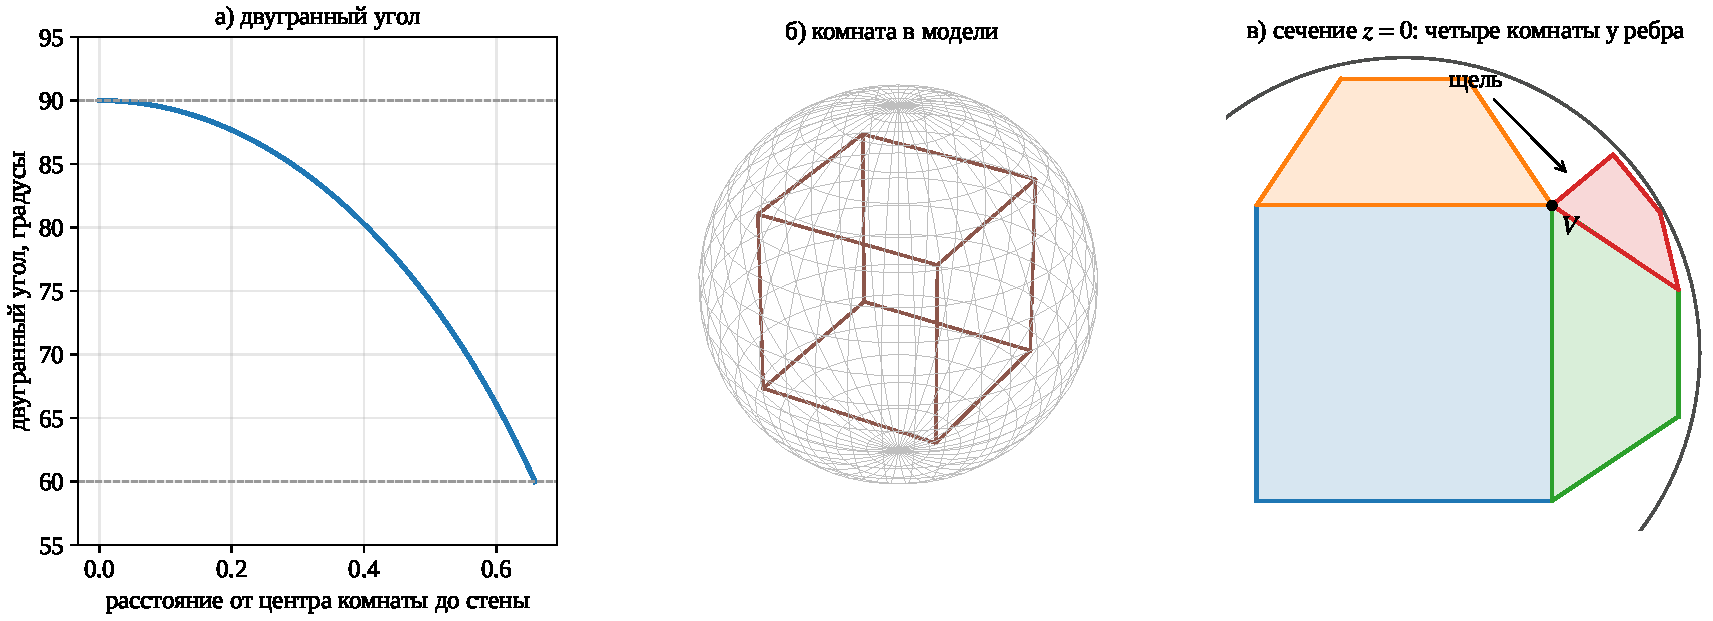
\includegraphics[width=\textwidth]{fig/kub.pdf}
\caption{Кубическая комната: а) двугранный угол в зависимости от расстояния от центра до стены; б) комната в модели при $t=0{,}5$; в) сечение плоскостью $z=0$: исходная комната (синяя) и три её отражения у вершины $V$; между красной и оранжевой остаётся щель}
\label{fig:kub}
\end{figure}

Теорема~\ref{thm:kub}~--- пространственный вариант отсутствия прямоугольников (п.~3.1): из шести плоских стен нельзя собрать комнату, у которой все углы прямые. Если у правильного многогранника с центром в центре шара грани лежат на расстоянии $h$ (в координатах модели) от центра, а нормали соседних граней образуют евклидов угол $\varphi$, то, повторяя доказательство, получаем
\begin{equation}\label{eq:mnogogrannik}
\cos\alpha=\frac{h^2-\cos\varphi}{1-h^2}.
\end{equation}

\subsection{Комнаты-додекаэдры}

Для правильного додекаэдра $\cos\varphi=1/\sqrt5$. По формуле~\eqref{eq:mnogogrannik} угол $\alpha$ становится прямым при $h^2=1/\sqrt5$, то есть $h=5^{-1/4}\approx0{,}6687$. Вершины такого додекаэдра в модели лежат на расстоянии $t\approx0{,}8415$ от центра шара, расстояние от центра до грани равно $\operatorname{arth}h\approx0{,}808$, до вершины~--- $\operatorname{arth}t\approx1{,}226$.

Двугранный угол $\pi/2$ означает, что вокруг каждого ребра сходятся ровно четыре таких додекаэдра. Отражая додекаэдр в его гранях, получают заполнение всего пространства Лобачевского прямоугольными додекаэдрами без щелей и наложений~[11]. Получается дом из одинаковых комнат с прямыми углами, только у каждой комнаты двенадцать стен, и каждая стена~--- правильный пятиугольник.

\subsection{Комната с полом-орисферой}

Есть и другой способ получить комнату с прямыми углами: отказаться от плоского пола. Пусть $\ell=(1,0,0,1)$; это точка $\omega=(0,0,1)$ абсолюта. Возьмём
\begin{itemize}
  \item пол~--- орисферу $\sk{X}{\ell}=-1$ с координатами $u=(u_1,u_2)$ из доказательства теоремы~\ref{thm:krivizna};
  \item потолок~--- концентрическую орисферу $\sk{X}{\ell}=-e^{-h}$;
  \item четыре стены~--- плоскости с полюсами
  \[
  P_{\pm1}=(\pm a,\,1,\,0,\,\pm a),\qquad P_{\pm2}=(\pm a,\,0,\,1,\,\pm a).
  \]
\end{itemize}

\begin{theorem}\label{thm:komnata}
У такой комнаты все двугранные углы между стенами, а также между стенами и полом или потолком прямые; противоположные стены параллельны. Пол~--- евклидов квадрат со стороной $2a$, который можно замостить евклидовыми квадратами, потолок~--- евклидов квадрат со стороной $2ae^{-h}$, высота комнаты равна $h$.
\end{theorem}
\begin{proof}
Все полюсы нормированы: $\sk{P_{\pm1}}{P_{\pm1}}=-a^2+1+a^2=1$. Каждый из них удовлетворяет условию $\sk{P}{\ell}=0$, поэтому точка $\ell$ лежит на каждой стене, и стены состоят из прямых связки параллельных прямых $B_\ell$. По теореме~\ref{thm:svyazka} эти прямые перпендикулярны полу и потолку, значит, перпендикулярны им и стены.

Точка пола $X(u)$ лежит на стене с полюсом $P_{\pm1}$ тогда и только тогда, когда
\[
\sk{X(u)}{P_{\pm1}}=\mp a+u_1=0,
\]
так как слагаемое с $|u|^2$ уничтожается благодаря $\sk{\ell}{P_{\pm1}}=0$. Значит, стены высекают на полу прямые $u_1=\pm a$, $u_2=\pm a$, и по теореме~\ref{thm:krivizna} пол~--- евклидов квадрат со стороной $2a$. Соседние стены перпендикулярны, так как $\sk{P_1}{P_2}=-a^2+a^2=0$; противоположные стены параллельны, так как $\sk{P_1}{P_{-1}}=a^2+1-a^2=1$ (п.~5.3). Наконец, по замечанию в конце п.~5.7 потолок лежит на расстоянии $h$ от пола по прямым связки, и длины на нём в $e^{h}$ раз меньше.
\end{proof}

Комната, все углы которой прямые, в пространстве Лобачевского существует, но за это приходится платить: пол и потолок у неё изогнуты, потому что это орисферы, и потолок меньше пола. Потолок вдвое меньше пола при высоте $h=\ln2\approx0{,}693$. Стены сходятся к точке $\omega$ на абсолюте, и в модели комната похожа на усечённую пирамиду с выпуклыми основаниями (рисунок~\ref{fig:komnata}).

\begin{figure}[H]
\centering
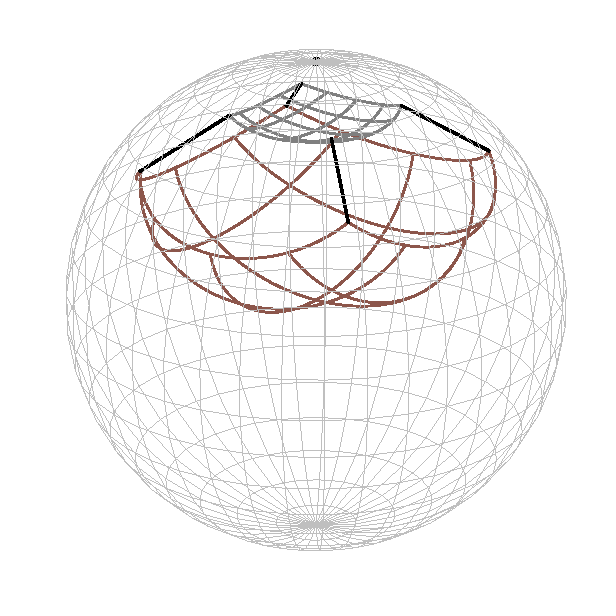
\includegraphics[width=0.6\textwidth]{fig/komnata.pdf}
\caption{Комната с полом-орисферой в модели: пол (коричневая сетка из евклидовых квадратов), потолок (серая сетка), четыре вертикальных ребра~--- прямые связки, сходящиеся в точке $\omega$ абсолюта; $a=1{,}2$, $h=0{,}9$}
\label{fig:komnata}
\end{figure}

\subsection{Интерактивная модель «Круг Кэли~--- Клейна»}

По формулам работы создана веб-страница «Круг Кэли~--- Клейна» (приложение~А). Она состоит из двадцати одной сцены: четырнадцать относятся к плоскости (разделы~1--4), семь~--- к пространству (разделы~5 и~6), и каждая посвящена одному утверждению или одной группе утверждений (таблица~\ref{tab:sceny}). В сценах на плоскости точки и концы хорд передвигаются мышью или пальцем, в сценах в пространстве рисунок можно поворачивать, а параметры задаются ползунками. Рядом с рисунком приведены формулировка утверждения, вычисленные величины и вопросы к сцене.

\begin{table}[H]
\caption{Сцены интерактивной модели}
\label{tab:sceny}
\centering
\singlespacing\footnotesize
\begin{tabular}{|c|>{\raggedright\arraybackslash}p{5.4cm}|>{\raggedright\arraybackslash}p{6.6cm}|c|}
\hline
№ & Сцена & Что показывает & Пункт \\ \hline
1 & Модель Кэли~--- Клейна & длина через сложное отношение, деления равной длины & 1.3 \\ \hline
2 & π-движения & сохранение длин и углов при переносе фигуры & 1.3 \\ \hline
3 & Аксиома Лобачевского & пучок прямых через точку, две параллельные & 2.1 \\ \hline
4 & Параллельность через внутренний луч & точка пересечения внутреннего луча с прямой уходит на абсолют & 2.1 \\ \hline
5 & Биссектраль и равнонаклонные & ось симметрии двух параллельных & 2.1 \\ \hline
6 & Функция Лобачевского & угол параллельности и его график & 2.2 \\ \hline
7 & Общий перпендикуляр и расстояние & построение через полюсы, график расстояния & 2.3, 2.4 \\ \hline
8 & Сумма углов и средняя линия & сумма углов, дефект, дополнительные построения & 3.1 \\ \hline
9 & Серединные перпендикуляры & треугольник и серединные перпендикуляры к его сторонам & 3.5 \\ \hline
10 & Двупрямоугольник и четырёхугольник Саккери & углы и стороны при изменении длин & 3.2 \\ \hline
11 & Окружность, эквидистанта, орицикл & оси, касательные, хорды & 3.3, 5.2 \\ \hline
12 & Острый угол и заградительная прямая & перпендикуляры к стороне угла, граничная точка & 3.4 \\ \hline
13 & Независимость аксиомы параллельности & евклидова плоскость и модель рядом & 4.2 \\ \hline
14 & Евклид и Лобачевский & сводный перечень утверждений со ссылками на сцены & --- \\ \hline
15 & Сфера & эллипсоид, изображение центра и евклидов центр, кривизна & 5.6, 5.7 \\ \hline
16 & От сферы к орисфере & сферы через одну точку с центром, уходящим к абсолюту & 5.5 \\ \hline
17 & Орисфера и её сетка & связка параллельных прямых, евклидова сетка на орисфере & 5.7 \\ \hline
18 & Эквидистантная поверхность & перпендикуляры к плоскости через её полюс & 5.6 \\ \hline
19 & Кубическая комната & двугранный угол и щель между четырьмя комнатами у ребра & 6.2 \\ \hline
20 & Комната-додекаэдр & прямой двугранный угол, четыре комнаты у ребра & 6.3 \\ \hline
21 & Комната с полом-орисферой & пол, потолок и стены, отношение сторон & 6.4 \\ \hline
\end{tabular}
\end{table}

Все величины на панели вычисляются по формулам разделов~1 и~5. Перпендикуляр строится через полюс (лемма~\ref{lem:polyus}), углы находятся по предложению~\ref{prop:ugol} или после переноса вершины в центр сдвигом~\eqref{eq:sdvig}, длины~--- по предложению~\ref{prop:ch}, симметрии~--- по формуле~\eqref{eq:otrazhenie}, окружности, эквидистанты и орициклы~--- по уравнениям~\eqref{eq:klein-traektoriya}. Перед публикацией вычислительное ядро проверено на 2000 случайных наборах точек. Длина через сложное отношение совпала с формулой~\eqref{eq:ch}, движения сохраняли длины и углы, угол между перпендикуляром, построенным через полюс, и прямой оказался прямым, точки построенных окружностей, эквидистант и орициклов лежали на нужном расстоянии; наибольшее отклонение во всех проверках не превысило $10^{-12}$. Страница написана на языке JavaScript и состоит из одного файла, поэтому её можно открыть в любом браузере, в том числе на телефоне.

Углы на рисунке модели искажены, и это одна из причин держать числа рядом с рисунком: трапеция на рисунке~\ref{fig:sakkeri} выглядит как евклидова, а её верхние углы равны $54{,}3^\circ$.

\subsection{Модели поверхностей на языке Python}

Модели гиперболической сферы и орисферы написаны также на языке Python с библиотеками Plotly и Dash (приложение~А). В модели сферы задаются гиперболический центр и гиперболический радиус $\rho$, а эллипсоид строится по формулам~\eqref{eq:sfera-poluosi}; хорды, проходящие через центр, пересекают его в точках, вычисленных по тем же формулам. Проверка на 48 наборах параметров показала, что все точки поверхности и все 2400 точек входа и выхода хорд удалены от центра на $\rho$ с точностью порядка $10^{-12}$. Модель орисферы использует параметр $k'$, связанный с полуосью формулой $r^2=k'/(1+k')$; в обозначениях п.~5.6 это $k'=c^2$.

Следующий шаг работы~--- модель комнаты, которую можно рассматривать изнутри. Её удобно строить тоже в модели Кэли~--- Клейна. Если наблюдатель находится в центре шара, направления на точки пространства изображаются без искажений, а перемещение наблюдателя заменяется π-движением всего пространства, то есть умножением однородных координат на матрицу, сохраняющую форму абсолюта. Видеокарта сама выполняет переход от однородных координат к точке шара, плоские грани остаются плоскими, и изображение получается точным; разбивать на мелкие части нужно только кривые поверхности, например пол-орисферу.
